\documentclass{ecnreport}

\stud{Control \& Robotics Master}
\topic{Manipulator Modeling \& Control}

\begin{document}
  
  \inserttitle{Manipulator Modeling \& Control}
  
  \section{Content of this lab}
  
  The goal of this lab is to program in C++ the three fundamentals models for robot manipulators:
  \begin{itemize}
    \item Direct Geometric Model: what is the pose of the end-effector for a given joint configuration?
    \item Inverse Geometric Model: what joint values correspond to a given end-effector pose?
    \item Kinematic Model: what is the velocity screw of the end-effector when the joints move?
  \end{itemize}
  These models will be applied on three different robots, and used to perform basic point-to-point control.\\
  
  As it is not a lab on C++, most of the code is already written and you only have to fill the required functions:
  \begin{itemize}
    \item \texttt{Robot::init\_wMe()} to initialize the fixed transform between the wrist and end-effector
    \item \texttt{Robot::fMw(q)} for the direct geometric model wrist-to-fixed frame
    \item \texttt{Robot::inverseGeometry(M)} for...well, the inverse geometry
    \item \texttt{Robot::fJw} for the kinematic model wrist-to-fixed frame
  \end{itemize}
  
  \subsection{Installing and loading the lab in Qt Creator}
  
  This project uses the ROS\footnote{Robot Operating System, http://www.ros.org} framework which imposes some particular steps to configure the environment. An actual ROS course will be held in the second semester, for now just configure as follows:
  
  \begin{enumerate}
    \item Open a terminal and create (if needed) a ROS workspace: \texttt{mkdir -p $\sim$/ros/src}
    \item Go inside this folder \texttt{cd $\sim$/ros/src}
    \item Download this repository: \texttt{git clone https://github.com/oKermorgant/ecn\_manip}.
    \item Compile the workspace: \texttt{cd .. \&\& catkin build}
    \item Create the QtCreator configuration file: \texttt{cd src/ecn\_manip \&\& gqt}
    \item Open QtCreator and load the \texttt{$\sim$/ros/src/ecn\_manip/CMakeLists.txt} file
    \item The files should be displayed and ready to run
    \item Compilation is done by clicking the bottom-left hammer
    \item Run your program with the green triangle. It can be stopped by clicking on the red square
  \end{enumerate}
  
  \subsection{Expected work}
  
  The {\bf only} files to be modified are:
  \begin{itemize}
    \item \texttt{control.cpp}: main file where the control is done depending on the current robot mode
    \item \texttt{robot\_turret.cpp}: model of the RRP turret robot
    \item \texttt{robot\_kr16.cpp}: model of the industrial Kuka KR16 robot
    \item \texttt{robot\_ur10.cpp}: model of the Universal Robot UR-10
  \end{itemize}
  We will use the ViSP\footnote{Visual Servoing Platform, http://visp.inria.fr} library to manipulate mathematical vectors and matrices, including frame transforms, rotations, etc. The main classes are detailed in Appendix \ref{visp}.\\
  At the end of the lab, you should upload them through the \link{http://pagesperso.ls2n.fr/~kermorgant-o/student links.php}{portal on my website}
  
  \section{The robots}
  
  \def\wMe{{}^w\M_e}
  
  Three robots are proposed with increasing complexity. You should start with the Turret, then the Kuka KR16 then the UR-10.\\
  For each of these robots, the table of Modified Denavit-Hartenberg parameters should be defined. As we saw during the lectures, once you have the table then the Direct Geometric and Direct Kinematic Models can be almost automatically derived. A tool is provided in this package to generate C++ code for the Geometric and Kinematic models, see Appendix \ref{dhcode} for details on this tool.
  
  The fixed frame and the end-effector frame are imposed by the schematics. 
  All intermediary frames have to be placed according to MDH convention, with a final fixed transform between the wrist and end-effector frames.
  
  \subsection{Turret RRP robot}
  
  \begin{minipage}{.8\linewidth}
    This is a very simple robot to begin the modeling, as shown in the figure.\\
    The fixed frame $\Frame{0}$ and end-effector frame $\Frame{e}$ are imposed, as well as the joint direction.\\
    The constant values for this model are: $b = 0.5$ m and $d = 0.1$ m.\\~\\
    All computation may be done first without using the Denavit-Hartenberg parameters as the robot is quite simple. 
  \end{minipage}
  \begin{minipage}{.2\linewidth}
    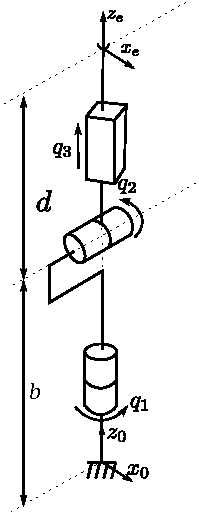
\includegraphics{fig/turret}\label{turret}
  \end{minipage}
  
  \subsection{Kuka KR16 anthropomorphic robot}
  
  This robot is a classical 6R architecture with a spherical wrist, as shown in the next figure:
  
  \begin{figure}[h!]\centering
    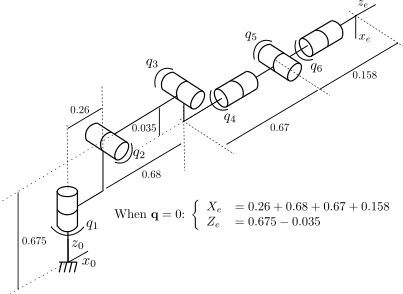
\includegraphics[width=.6\linewidth]{fig/kr16}
    \caption{Model of the Kuka KR16 with imposed fixed and end-effector frames}
  \end{figure}
  
  The wrist frame is typically at the common point between joints 4, 5 and 6.
  The constant transform $\wMe$ between the wrist and the end-effector should include the $0.158$ distance and potential rotations.
  
  \subsection{Universal Robot UR-10 anthropomorphic robot}
  
  This robot is a less classical 6R architecture, without spherical wrist. A tool is also attached with an arbitrary end-effector offset.
  
  \begin{figure}[h!]\centering
    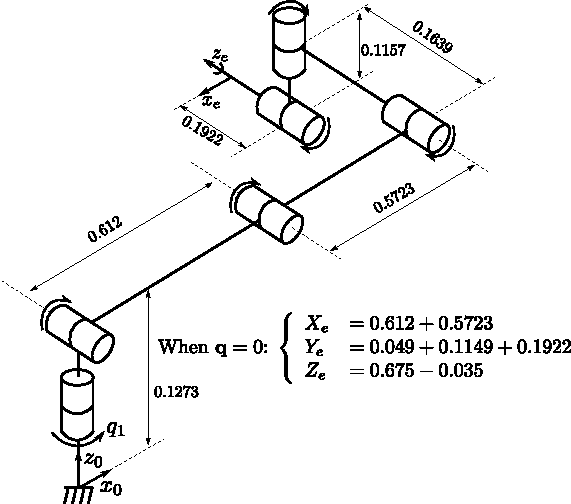
\includegraphics[width=.6\linewidth]{fig/ur10}
    \caption{Model of the UR-10 with imposed fixed and end-effector frames}
  \end{figure}
  
  The Inverse Geometry is given for this robot. 
  The constant transform $\wMe$ between the wrist and the end-effector should include the $0.1922$ distance and potential rotations.
  
  
  \newpage
  \subsection{Running the simulation}
  
  Once everything is installed and compiled, the base simulation can be run from a terminal (only 1 line depending on the robot you work on):
  \cppstyle
  \begin{lstlisting}
  roslaunch ecn_manip turret.launch
  roslaunch ecn_manip kr16.launch
  roslaunch ecn_manip ur10.launch
  \end{lstlisting}
  
  This will display two windows:
  \begin{itemize}
    \item RViz is the 3D simulator to show the current configuration of the robot. It will also display the base and end-effector frames, and the one that you compute. You can thus easily check if the computation is fine.
    \item The other window is composed of 4 panels:
    \begin{itemize}
      \item Buttons at the top left to change the current exercise
      \item Sliders at the bottom left to manually control the robot (exercises 1 and 2)
      \item Sliders at the top to change the switching time of the position control (exercises 3+)
      \item A plotting region with two tabs, one for the operational space and one for the joint space. The joint space is displayed in a normalized fashion, depending on the joint limits (upper and lower dotted lines)
    \end{itemize}
  \end{itemize}
  
  
  \section{Building the models}
  
  \subsection*{The main code}
  
  In the file \texttt{control.cpp}, the \texttt{if - else if} blocks correspond to the 6 exercises to be done for each robot. Note that if they work for the Turret robot, then 
  they should work for all robots as long as the model is correct. \\
  The current exercise is changed by using the buttons in the GUI.
  
  \subsection*{Exercise 1: Checking the Direct Geometric Model}
  
  In this exercise, the robot follows the manually given joint positions. The task is to build and print the direct geometric model, depending on the current value of $\q$. This is to be done in two functions:
  \begin{itemize}
    \item \texttt{Robot::init\_wMe()} where you have to write the constant matrix $\wMe$ from the end-effector to the wrist frame
    \item \texttt{Robot::fMw(q)}  where you have to write and return the transform $\M$ between the fixed and wrist frame
  \end{itemize}
  Once you have computed the \texttt{M} matrix, the code calls \texttt{robot->checkPose(M);} in order to print both your matrix and the true one. No need to tell that they should be equal.\\
  What can be told is that it is useless to continue until they are.
  
  \subsection*{Exercise 2: Checking the Direct Kinematic Model (Jacobian)}
  
  If you select \texttt{Manual Operational Velocity} in the GUI then the sliders allow you to give a desired operational velocity (ie twist) for the end-effector.\\
  This velocity is ${}^e\v_e$ and is defined in the end-effector frame.\\
  The robot Jacobian has to be defined in the function \texttt{Robot::fJw(q)} that should return the Jacobian of the wrist in the fixed frame.\\
  
  
  In the main code, the commanded velocity then to be mapped to the joint velocity in two steps:
  \begin{enumerate}
    \item Map to the fixed frame: ${}^f\mathbf{v}_e^* = \left[\begin{array}{cc}{}^f\R_e & 0 \\ 0 & {}^f\R_e\end{array}\right]{}^e\mathbf{v}_e^*$\\
    Call \texttt{M.getRotationMatrix()} to get this rotation.\\
    The \texttt{ecn::putAt} function may be of good use.
    \item Map to the joint space: $\dot\q = \J^+.{}^f\mathbf{v}_e^*$\\
    Call \texttt{robot->fJe(q).pseudoInverse()} to get the Jacobian pseudo-inverse
  \end{enumerate}
  You can check that the end-effector is able to follow straight 3D lines in x, y or z direction in its own frame.
  Similarly, it should be able to rotate around x, y or z. This means the Jacobian computation is correct.
  
  \newpage
  \subsection*{Exercise 3: Checking the Inverse Geometric Model}
  
  If you select \texttt{Direct point-to-point} in the GUI then the robot will receive two operational setpoints, at a given sampling time that can be changed with the \texttt{Switching time} slider in the GUI. The current setpoint is in the matrix \texttt{Md} and its corresponding joint position is in the vector \texttt{qf}. 
  
  Nothing has to be done in the main code, but of course the \texttt{Robot::inverseGeometry(M)} function has to be filled in order to compute the actual inverse geometry solution. The robot will try to have all joints reach their desired value as soon as possible, which will lead to a discontinuous motion.\\
  
  In practice, this exercise is to check that the Inverse Geometric Model is correct: the robot should reach the desired pose.\\
  
  When computing the inverse geometry, try to find a solution as near as possible to the passed \texttt{q0}.\\
  
  Many useful functions are available to solve classical trigonometric equations. They are detailed in Appendix \ref{trigsolve}.\\
  
  A given potential solution should be stored using \texttt{addCandidate(\{q1, q2, ..., qn\});}\\ At the end of the Inverse Geometry function, use \texttt{return bestCandidate(q0);} that will pick the candidate that is the nearest from the current joint position and also within joint limits.
  
  \subsection*{Exercise 4: Interpolated point-to-point control}
  
  In this exercise the previous pose setpoint \texttt{M0} and its corresponding joint position \texttt{q0} should be used to interpolate the joint positions.\\
  
  Here the goal is to compute the current setpoint $\q_c = \q_0 + p(t)(\q_f-\q_0)$. The interpolation function $p(t)$ was defined during the lectures and should take into account the maximum joint velocity and acceleration that are stored in the \texttt{vMax} and \texttt{aMax} vectors. Basically this amounts to computing the minimum time \texttt{tf} needed to reach $\q_f$ from $\q_0$. This computation should be done in the \texttt{if(robot->newRef())} and then used to compute the current \texttt{qCommand}.
  
  
  \subsection*{Exercise 5: Operational control through Inverse Geometric Model}
  
  Exercises 3 and 4 lead to the correct pose but not in a straight 3D line. Indeed the robot is only controlled in the joint space with no constraints between the two extreme poses.\\
  In this exercise, the goal is to perform the interpolation not in the joint space but in the Cartesian space. In practice, we will compute many poses between 
  \texttt{M0} and \texttt{Md} and command the robot to reach sequentially all these poses. As they will be pretty close one from each other, the resulting motion 
  will be close to a straight line.
  
  The \texttt{robot->intermediaryPose(M0, Md, alpha)} function returns a pose between \texttt{M0} and \texttt{Md}, where \texttt{alpha} is between 0 and 1 and should be computed from $t$, $t_0$ and $t_f$ = 1 s.
  
  Then, the inverse geometry of this pose should be sent to the robot as joint position setpoint.
  
  \newpage
  \subsection*{Exercise 6: Operational control through Jacobian}
  
  In this exercise the goal is still to follow a straight line between the two points, but this time by sending a joint velocity command.\\
  
  As seen in class, this command should make the end-effector approach its desired pose. The steps are:
  \begin{enumerate}
    \item Compute the pose error in the desired frame: ${}^{e*}\M_e = {}^{f}\M_{e*}^{-1}.{}^{f}\M_e$
    \begin{itemize}
      \item in the code, ${}^{f}\M_{e*}$ corresponds to \texttt{Md} and ${}^{f}\M_e$ to \texttt{M} 
      \item In practice we use the $(\mathbf{t}, \theta\u)$ representation with \texttt{p.buildFrom()}
    \end{itemize}
    \item Compute the desired linear and angular velocities: $v = -\lambda{}^{f}\M_{e*}\mathbf{t}$, \quad $\omega = -\lambda{}^{f}\M_{e} (\theta\u)$
    \item Map these velocities to the joint space: $\dot\q = \J^+ \left[\begin{array}{c}v\\\omega\end{array}\right]$
  \end{enumerate}
  $\lambda$ is a gain that can be changed from the GUI. Increasing it will lead to a faster convergence. It can be obtained through \texttt{robot->lambda()}.
  
  
  
  \appendix
  
  
  \newpage
  
  \section{Using ViSP}\label{visp}
  
  ViSP is a library for Visual Servoing (wait for the M2 Robotics to know more!) and also includes all necessary tools to play with mathematical vectors, matrices and 3D transforms.
  The full documentation is here: \link{http://visp-doc.inria.fr/doxygen/visp-3.1.0/classes.html}{http://visp-doc.inria.fr/doxygen/visp-3.1.0/classes.html}.\\
  The main classes to be used are:
  \begin{itemize}
    \item \texttt{vpMatrix}: a classical matrix of given dimensions, can be multiplied with other matrices and vectors if the dimensions are ok. The pseudo-inverse of matrix \texttt{M} 
    is available with \texttt{M.pseudoInverse()}
    \item \texttt{vpColVector}: a column vector of given dimension
    \item \texttt{vpHomogeneousMatrix}: the classical $4\times 4$ 3D transform matrix
  \end{itemize}
  Most of the model computation is about initializing a matrix or vector to correct dimensions (which is already done) and fill its elements with formulae.\\
  To write 1 at element (i,j) of matrix M, just write \texttt{M[i][j] = 1;}\\
  Similarly, to write 1 at element (i) of vector q, just write \texttt{q[i] = 1;}\\
  
  3D transforms can be easily changed between homogeneous matrix, rotation matrix, translation vector or $\theta\u$ vector. Another type called a pose vector
  consists in the full $(\mathbf{t}, \theta\u)$ vector of dimension 6:
  \cppstyle
  \begin{lstlisting}
  vpHomogeneousMatrix M;
  vpPoseVector p;
  vpRotationMatrix R;
  vpTranslationVector t;
  vpColVector tu(3);
  
  M.getRotationMatrix()*t;	// extract the rotation part from M and multiply with t
  p.buildFrom(M);			// build (t, theta-u) from M
  t = M.getTranslationVector();	// extract the translation part
  
  // copy the theta-u part of p into tu
  for(int i = 0; i < 3; ++i)
  tu[i] = p[i+3];
  
  // compute inverse transform
  M = M.inverse();
  \end{lstlisting}
  
  Two utility functions are provided to put a matrix or vector into a bigger one:
  \begin{itemize}
    \item \texttt{void ecn::putAt(M, Ms, r, c)}: Writes matrix \texttt{Ms} inside matrix \texttt{M}, starting from given row and column.
    \item \texttt{void ecn::putAt(V, Vs, r)}: Writes column vector \texttt{Vs} inside vector \texttt{V}, starting from given row. These two functions do nothing but print an error
    if the submatrix or vector does not fit in the main one.
  \end{itemize}
  
  
  \newpage
  \section{Code generation from Modified Denavit-Hartenberg parameters}\label{dhcode}
  
  The core of robot modeling is to build the MDH table. From this, the DGM and KM can be derived automatically. The Inverse Geometry still has to be done by hand (even if some advanced tools allow code-generation for the IG resolution).
  
  As it is quite tedious to have to compute all matrices when a solution of MDH is investigated, a tool is provided to generate the C++ code. An example can be found in the file \texttt{dh\_example.yml}:
  \cppstyle
  \begin{lstlisting}
  notation: [alpha, a, theta, r]
  joint:
  1: [0, 0, q1, 0]
  2: [-pi/2, 0, 0, q2]
  3: [pi/2, 0, q3, r3]
  4: [-pi/2, a4, q4+pi/2, 0]
  \end{lstlisting}
  The command to be run is: \texttt{rosrun ecn\_manip dh\_code.py <name of the file>}.\\
  In the case of the above MDH table, it leads to these outputs:
  
  \begin{minipage}{.45\linewidth}
    \cppstyle \raggedright
    \begin{lstlisting}
    // Generated pose code                                                                                                                                                                                                                  
    const double c1 = cos(q[0]);                                                                                                                                                                                                            
    const double c1p3 = cos(q[0]+q[2]);                                                                                                                                                                                                     
    const double c4 = cos(q[3]);                                                                                                                                                                                                            
    const double s1 = sin(q[0]);                                                                                                                                                                                                            
    const double s1p3 = sin(q[0]+q[2]);                                                                                                                                                                                                     
    const double s4 = sin(q[3]);                                                                                                                                                                                                            
    M[0][0] = -s4*c1p3;                                                                                                                                                                                                                     
    M[0][1] = -c4*c1p3;                                                                                                                                                                                                                     
    M[0][2] = -s1p3;                                                                                                                                                                                                                        
    M[0][3] = a4*c1p3 - q[1]*s1;                                                                                                                                                                                                            
    M[1][0] = -s4*s1p3;
    M[1][1] = -s1p3*c4;
    M[1][2] = c1p3;
    M[1][3] = a4*s1p3 + q[1]*c1;
    M[2][0] = -c4;
    M[2][1] = s4;
    M[2][2] = 0;
    M[2][3] = r3;
    M[3][0] = 0;
    M[3][1] = 0;
    M[3][2] = 0;
    M[3][3] = 1.;
    // End of pose code
    \end{lstlisting}
  \end{minipage}
  \begin{minipage}{.1\linewidth}
    \quad\quad
  \end{minipage}
  \begin{minipage}{.45\linewidth}
    \cppstyle \raggedright
    \begin{lstlisting}
    // Generated Jacobian code
    const double c1 = cos(q[0]);
    const double c1p3 = cos(q[0]+q[2]);
    const double s1 = sin(q[0]);
    const double s1p3 = sin(q[0]+q[2]);
    J[0][0] = -a4*s1p3 - q[1]*c1;
    J[0][1] = -s1;
    J[0][2] = -a4*s1p3;
    //J[0][3] = 0;
    J[1][0] = a4*c1p3 - q[1]*s1;
    J[1][1] = c1;
    J[1][2] = a4*c1p3;
    //J[1][3] = 0;
    //J[2][0] = 0;
    //J[2][1] = 0;
    //J[2][2] = 0;
    //J[2][3] = 0;
    //J[3][0] = 0;
    //J[3][1] = 0;
    //J[3][2] = 0;
    J[3][3] = -s1p3;
    //J[4][0] = 0;
    //J[4][1] = 0;
    //J[4][2] = 0;
    J[4][3] = c1p3;
    J[5][0] = 1.;
    //J[5][1] = 0;
    J[5][2] = 1.;
    //J[5][3] = 0;
    // End of Jacobian code
    \end{lstlisting}	
  \end{minipage}
  This is exactly what you would get by doing the manual computation from the initial table, which I hope is quite appreciated.\\
  
  Fixed transforms for initial and end-effector frames can also be written with keys \texttt{f:} and \texttt{e:}\\
  
  If passing \texttt{--display} the script will display the direct geometry with classical math notations. It can be useful for the inverse geometry computation.\\
  For a 6-DOF robot, passing \texttt{--wrist} will display useful information to benefit from a spherical wrist: math expressions for $\Pass{0}{\mathbf{t}}{6}(q_1,q_2,q_3)$ and  $\Pass{3}{\R}{6}(q_4,q_5,q_6)$, and code for $\Pass{0}{\R}{3}(q_1,q_2,q_3)$.
  
  \newpage
  \section{Trigonometric solvers}\label{trigsolve}
  
  The code contains solvers for all types of trigonometric equations (except type 1 that is obvious).\\
  They take as argument the coefficients of the equations. They return:
  \begin{itemize}
    \item A \texttt{std::vector<double>} for equations of 1 unknown (types 2 \& 3).\\We can go through the valid solutions with:
    \cppstyle
    \begin{lstlisting}
    // assume q1 should ensure type 2: X.sin(q1) + Y.cos(q1) = Z
    
    for(double q1: solveType2(X, Y, Z))
    {
    // here q1 is a valid solution, may be used to deduce other joint values
    }
    \end{lstlisting}
    \item A \texttt{std::vector<JointSolution>} for equations of 2 unknowns (types 4 to 8).\\In this case, the valid solutions can be explored with:
    \cppstyle
    \begin{lstlisting}
    // assume q1 and q2 should ensure type 6 equation: 
    //		W.sin(q2) = X.cos(q1) + Y.sin(q1) - Z1
    //		W.cos(q2) = X.sin(q1) - Y.cos(q1) - Z1
    
    for(auto qs: solveType6(X, Y, Z1, Z2, W))
    {
    // here a (q1,q2) solution is available in qs.qi and qs.qj
    }
    \end{lstlisting}
  \end{itemize}
  
  Furthermore, a function allows retrieving the 12 elements of $\Pass{0}{\M}{n*}$ from the matrix $\Pass{f}{\M}{e*}$ given to the inverse geometry solver:
  \begin{cppcode}
    const auto [xx,xy,xz,yx,yy,yz,zx,zy,zz,tx,ty,tz] = explodeMatrix(fMe_des);
\end{cppcode}
This function output the matrix terms according to:
\begin{equation*}
\Hom{0}{n*} = \Hom{0}{f}\Hom{f}{e*}\Hom{e}{n} = \left[\begin{matrix}x_x & y_x & z_x & t_x\\x_y & y_y & z_y & t_y\\x_z & y_z & z_z & t_z\\0 & 0 & 0 & 1\end{matrix}\right] 
\end{equation*}


  
  \newpage
  Below are listed the syntax for all trigonometric solvers:\\
  
  %\setlength\extrarowheight{5pt}
  \renewcommand{\arraystretch}{2.2}
  \begin{tabular}{|c|c|C{7cm}|C{2cm}|}\hline
    Type & Equation & Syntax & Returns (vector of)\\\hline
    1 & $Xq_i = Y$& does not exist &$q_i$	\\\hline		
    2 & $Xs_i+Yc_i = Z$ & \texttt{solveType2(x, y, z)}&$q_i$\\\hline
    3 & $\begin{array}{l}X_1s_i+Y_1c_i = Z_1 \\ X_2s_i+Y_2c_i = Z_2\end{array}$&\texttt{solveType3(x1, y1, z1,
      x2, y2, z2)} &$q_i$\\\hline
    4 & $\begin{array}{l}X_1q_js_i = Y_1 \\ X_2q_jc_i = Y_2\end{array}$& \texttt{solveType4(x1, y1, x2, y2)}&$(q_i,q_j)$ \\\hline
    5 & $\begin{array}{l}X_1s_i = Y_1+Z_1q_j \\ X_2c_i = Y_2+Z_2q_j\end{array}$& \texttt{solveType5(x1, y1, z1,
      x2, y2, z2)}&$(q_i,q_j)$\\\hline			
    6 & $\begin{array}{l}Ws_j = Xc_i + Ys_i+Z_1 \\ Wc_j = Xs_i - Yc_i+Z_2\end{array}$& \texttt{solveType6(x, y,
      z1, z2, w)}&$(q_i,q_j)$\\\hline
    7 & $\begin{array}{l}W_1c_j +W_2s_j = Xc_i + Ys_i+Z_1 \\ W_1s_j -W_2c_j = Xs_i - Yc_i+Z_2\end{array}$& \texttt{solveType7(x, y, z1, z2, w1, w2)}&$(q_i,q_j)$\\\hline
    8 &$\begin{array}{l}Xc_i+Yc_{ij} =Z_1 \\ Xs_i+Ys_{ij} =Z_2\end{array}$ & \texttt{solveType8(x, y, z1, z2)}&$(q_i,q_j)$\\\hline
  \end{tabular}
  
  
\end{document}
